\documentclass{IEEEtran}
\usepackage[utf8]{inputenc}
\usepackage[T1]{fontenc}
\usepackage[ngerman]{babel}
\usepackage{acronym}
\usepackage{footnote}
\usepackage{algorithmic}
\usepackage{graphicx}
\usepackage[autostyle=true,german=quotes]{csquotes}
\usepackage{todonotes}
 

\usepackage{hyperref}

\long\def\comment / *#1* /{}

\begin{document}


\title{cowbus -- a small home automation bus}
\author{Robin~Backhaus \and Patrick~Kanzler \and Josef~Schnurrer \and Michael~Zapf}
\date{\today}



\maketitle

\begin{abstract}
\todo{formulieren}
    - Riot OS
    - STM32F0
    - nrf24l01+
    - offenes System
    - ziel: Einbindung in openHAB
\end{abstract}


\section{Einleitung}
    \enquote{Smart Home} ist ein Schlagwort, um das man im 21. Jahrhundert
    kaum noch herum kommt. Der moderne Mensch möchte sein Zuhause vernetzen.
    Lichtschalter sind nicht mehr nur noch passive Komponenten in einer
    Elektroinstallation, sie sind aktive Kommunikationspartner in einem großen Netz.
    Das Licht wird nicht nur am Schalter, sondern bequem von der Couch aus mit dem
    Smartphone, automatisch durch Sensoren oder zu einer bestimmten Uhrzeit geschalten. 
    Eingehende E-Mails erscheinen nebenbei im Fernsehbild, die Verdunklung fährt 
    automatisch herunter sobald die Sonne blendet --
    all das ist keine Science Fiction mehr sondern längst Realität.

\section{Motivaton}
    Die meißten erhältlichen \enquote{Smart Home}-Lösungen sind teuer und nicht offen.
    Da die Beliebtheit solcher Systeme immer größer wird, wäre eine größere 
    Zugänglichkeit durch günstige Alternativen und langfristige Sicherheit, 
    sowie mehr Kontrolle für und durch den Anwender wünschenswert.
    Unser Fokus liegt daher auf modernen, offenen Standards und einer drahtlosen, 
    flexiblen und damit einfach zu erweiternden Netzwerktopologie.
    Mit möglichst günstigen Komponenten sollen dabei Sensoren und Aktoren 
    mit verschiedensten Funktionen ermöglicht werden.
    Eine Anknüpfung an vorhandene IP-basierende Netze durch Gateways würde die 
    Anwendungsmöglichkeiten zusätzlich erhöhen 
    und es ermöglichen bereits bestehende und neue externe Anwendungen mit dem 
    cowbus zu verbinden.

\section{Projektidee und -ziele}
    Angefangen hat der cowbus mit der Suche nach einem Projekt für die Vorlesung 
    \enquote{DIY: Personal Fabrication} 2014/2015 von Dr.-Ing. Jürgen Eckert, durch 
    Michael Zapf und Patrick Kanzler. Im Rahmen der Veranstaltung hat sich dann ein 
    Team gebildet, um eine günstige, offene Alternative zu bestehenden Heimbussystemen 
    zu entwickeln. Das Team besteht aus Michael Zapf, Patrick Kanzler, Josef Schnurrer 
    und Robin Backhaus. 

    An zentraler Stelle des Projektes steht die Kommunikation zwischen Netzwerkknoten 
    und ein Netzwerkmodell, dass möglichst flexibel erweiterbar und verkleinerbar 
    sein soll. 
    Dazu wird ein drahtloses Mesh-Netzwerk mit dezentraler Organisation implementiert 
    und an Beispiel-Sensoren und -Aktoren getestet. 
    Als besonderes Merkmal soll das System aus einzelnen, kostengünstigen, sich 
    selbst vermaschenden Knoten bestehen.
    Die Sensoren und Aktoren sollen Ereignisse erzeugen und darauf reagieren können. 
    Optional könnte nach ersten Funktionstests der ausgewählten Hardware oder im 
    Anschluss an die erfolgreiche Implementierung eines Netzwerkes der Standart 
    \enquote{6LoWPAN} implementiert werden. 
    Um keine unbrauchbare Insellösung zu entwickeln, soll neben den Aktoren und 
    Sensoren ein Ethernet-Gateway implementiert werden. Durch dieses soll das 
    Meshnetzwerk als optionales Anwendungsbeispiel eine Verbindung zu 
    einer \enquote{OpenHAB}-Instanz aufnehmen können.


\section{Projektverlauf und Meilensteine}
    \subsection{Erstes Brainstorming}
    Die Wahl des Projektnamen fiel nicht leicht. Wir haben uns darauf geeinigt, dass 
    wir das Projekt DIY14BUS nennen und auch so anmelden. Nachdem wir im 
    Projektverlauf mehr über Technologie und Funktionsumfang festlegen, wollten wir 
    später einen "richtigen" Namen wählen. Die Wahl viel dann auf cowbus.

    Über die Implementierung von \enquote{6LoWPAN} waren wir uns nach einem ersten 
    Brainstorming nicht mehr sicher. Obwohl dies als moderner offener Standard 
    sehr wünschenswert war, hatten wir aufgrund der begrenzten Projektzeit Bedenken 
    zu viel Zeit zu verlieren wenn die Implementierung nicht auf Anhieb gelingen 
    sollte. Vorher ein funktionierendes Mesh-Netzwerk mit den von uns gewünschten 
    Eigenschaften zu implementieren erschien uns als wichtiger, vor allem um 
    eigene Erfahrungen zu sammeln. Wir entschieden uns dafür \enquote{6LoWPAN} 
    nicht sofort zu implementieren, sondern als Option für eine Weiterentwicklung 
    nach dem Projekt offen zu halten.

    Durch die Konkretisierung unserer Projektziele entschieden wir uns eine 
    \enquote{proof-of-work}-Herangehensweise zu wählen und als erstes unser 
    Sensor-Actor-Konzept umzusetzen. Erst im Anschluss sollte ein 
    Ethernet-Gateway folgen um den Funktionsumfang des cowbus zu erhöhen.

    \subsection{Projektplanung}
    Zeitlich haben wir das Projekt in Monate aufgeteilt. Für den restlichen Oktober 
    gaben wir uns Zeit uns kennen zu lernen, Informationen und Wissen über bestehende 
    und zu verwendende Technologien auszutauschen und uns in das Thema einzuarbeiten.
    Verwendete Software und Hilfsmittel sollten unter anderen GitHub, KiCad, JLink 
    und OpenOCD, sowie ein Blog zur Projektdokumentation sein, die für unsere 
    Projektinfrastruktur vorbereitet wurden.
    Im November sollten die ersten Tests und Anpassungen von RIOT OS in Verbindung 
    mit den Discovery-Boards stattfinden um anschließend mit der Planung und einem 
    Entwurf für unser Mesh-Netzwerk beginnen zu können.
    Nachdem unsere \enquote{nrf24l01+}-Funkchips angekommen waren sollte im Dezember 
    die Softwareentwicklung und  Funktests mit Discovery-Boards vorangehen, hier 
    stießen wir jedoch auf Komplikationen bei der Unterstützung durch RIOT OS. 
    Während wir dennoch unser erstes Funksignal übertragen konnten, gewannen wir 
    einen genaueren Überblick, welchen Funktionsumfang wir mit unseren 
    Sensor-Aktor-Prototypen im Rahmen des Projektes realisieren könnten, was die 
    Grundlage für das gleichzeitig stattfindende Schaltungslayout und 
    Platinendesign für unseren Prototypen sein sollte.
    Im Januar wollten wir die bisherigen Ergebnisse zusammenbringen und  
    Implementierung und Test der bisherigen Software am Prototypen vorantreiben. 
    Als Meilenstein nahmen wir uns vor in der Zwischenstandspräsentation erste 
    Showcases vorführen zu können. Unser Prototyp sollte als der 
    \enquote{Beispielknoten} gleichzeitig Sensor- (über Druckknöpfe) und 
    Aktorfunktionalitätten (verschiedene LEDs) haben.
    Für Februar hatten wir uns vorgenommen das Projekt soweit abzurunden und 
    unseren Schwerpunkt auf Fehlerbehebungen zu legen. Außerdem steht es noch an 
    die Arbeit an optionalen Projektzielen fortzuführen. 

    \subsection{Kennenlernen von RIOT OS}
    Um das Rad nicht neu zu erfinden, bietet es sich an, ein eingebettetes 
    Betriebssystem auf den Knoten einzusetzen. Relativ früh wurde uns der Tipp 
    gegeben, "RIOT OS" anzuschauen. \url{http://www.riot-os.org/} 
    \enquote{The friendly Operating System for the Internet of Things.}
    RIOT OS ist ein Betriebssystem für den Bereich embedded, welches auf das 
    Thema Internet of Things optimiert wurde. 
    Damit bietet es gegenüber Konkurrenten, wie chibiOS oder FreeRTOS den Vorteil, 
    dass einiges, wie eine saubere Netzwerkkommunikation mit Unterstützung für 
    IPv6 bereits implementiert ist. 
    Es soll 6LoWPAN zum Einsatz kommen, um auf den doch relativ schwachen 
    Knotengeräten Ressourcen zu sparen.
    Riot OS unterstützt Multithreading und ist aufgrund seiner Schichtenarchitektur
    gut portierbar. Eine Anwendung kann für unterschiedlichen Boards mit unterschiedlichen
    CPU-Kernen gleich geschrieben werden, da sich der Programmierer nicht um Hardware-Details
    kümmern muss. Dies ist dank der gut ausgeprägten Hardware Abstraction Layer (HAL), 
    die für jedes Board erstellt werden muss, möglich.
    Riot steht unter der LGPLv2 Lizenz.

    \subsection{Funkchip nrf24l01+}
    Die Wahl des Funkchips stand nach kurzer Recherche fest: Der nrf24l01+ von 
    Nordic Semiconductor. Der Transceiver ist günstig in der Anschaffung, da er 
    im zehner-Pack nur rund 1~Euro pro Stück kostet. Er arbeitet im 2,4GHz 
    ISM-Band, überträgt eine bis zu 2Mbps und ist bereits auf einer handlichen 
    kleinen Platine bestückt. Der Nachteil dieses Funkchips war jedoch die lange 
    Lieferzeit und der Treiber war in Riot OS nicht vorhanden.
    Um dennoch zügig mit der Entwicklung beginnen zu können, haben wurden erste 
    Versuche mit dem CC1101 von Texas Instruments gestartet, dessen Treiber 
    bereits in Riot vorhanden war. Parallel dazu haben wir den Treiber für den 
    nrf24l01+ Transceiver geschrieben. Trotz zweigleisiger Entwicklung ging der 
    Fortschritt nur stockend voran aufgrund der langen Einarbeitungszeit in Riot.

    \subsection{Erstes Prototyping mit Discovery Boards}
    Um die prinzipielle Funktionsweise überprüfen zu können, haben wir die 
    Transceiver an STM32F3-Discovery Boards angesteckt. Die Discovery Boards 
    sind Evaluationsplatinen für den STM32F3 ARM Prozessor von ST. Die Boards 
    können über den St-Link programmiert werden.
    Zwar werden die Discovery-Boards von Riot bereits unterstützt, jedoch war 
    für das F3-Board der SPI-Treiber zur Kommunikation mit dem Funk-Modul nicht 
    implementiert und musste mit Hilfe der Implementierungen der anderen 
    unterstützten Boards implementiert werden.

    \subsection{Erste Funkübertragung und Messung der Funkreichweite}
        Nach etwa der Hälfte der bisherigen Entwicklungszeit ist in Riot 
        glücklicherweise der Treiber für den nrf24l01+ Chip erschienen. Mit 
        diesem Treiber ist es erstmals gelungen, Pakete mit Riot zu versenden 
        und mit einem anderen Board zu empfangen.
        Der Treiber ist allerdings nicht in die bisherigen Module des 
        Netzwerkstapels integriert worden. Da die Integration zu aufwändig 
        gewesen wäre, wurde auf diesem Treiber aufgebaut und ein eigenes 
        Protokoll entworfen.

    \subsection{Platinendesign des Prototypes}
    An dieser Stelle erschienen drei Baustellen. Zum einen sollte ein Prototyp, 
    der cowbus-one, geplant und erstellt werden. Auf einer runden Platine soll 
    ein ARM-Prozessor von ARM, eine RGB-LED, und drei Taster platziert werden. 
    Dafür wurde erst der Schaltplan, dann das Layout erstellt und anschließend 
    die Platine gefertigt und bestückt.
    Die zweite Baustelle war die Hardware Abstraction Layer (HAL) von Riot OS 
    für unseren Prototypen. Als drittes sollte das entworfene Protokoll 
    implementiert werden, das im weiteren im Detail beschrieben wird.

 %   \subsection{Zwischenpresentation}

\section{Systemaufbau}
    \todo{Einleitung}

    \subsection{Funkmedium}
        Als Übertragungsmedium kommt eine $2,4~GHz$-Technologie
        zum Einsatz. Eine Funktechnologie eignet sich besonders gut dazu
        bereits bestehende Installationen um intelligente Komponenten
        zu erweitern, ohne größere bauliche Änderungen vornehmen zu müssen.

        Die Wahl eines ISM-Frequenzbandes (\enquote{Industrial, Scientific and Medical Band})
        ist in erster Linie bedingt durch die gute Verfügbarkeit von günstigen
        Systemkomponenten und der weltweiten Einsetzbarkeit ohne Anpassung der
        genutzten Frequenzen.

        Genutzt wird der Funkkanal im Moment als Broadcastmedium.
        Jeder Knoten kann also prinzipiell jedes Paket sehen und verarbeiten.
        Dies spart für den Anfang sehr viel Logik und Routingaufwand,
        da Pakete einfach ins Netz geflutet werden können und der entsprechende
        Empfänger (wobei das durchaus mehrere Knoten sein können -- ein Schalter
        könnte beliebig viele Lampen schalten) selbst an der Adresse erkennen
        kann, dass er darauf reagieren muss.

    \subsection{Komponenten}
        Grundsätzlich besteht der cowbus aus drei Typen von Komponenten,
        die auch in Abb. \ref{fig:comp} schematisch dargestellt sind.

        \begin{figure}
            \centering
            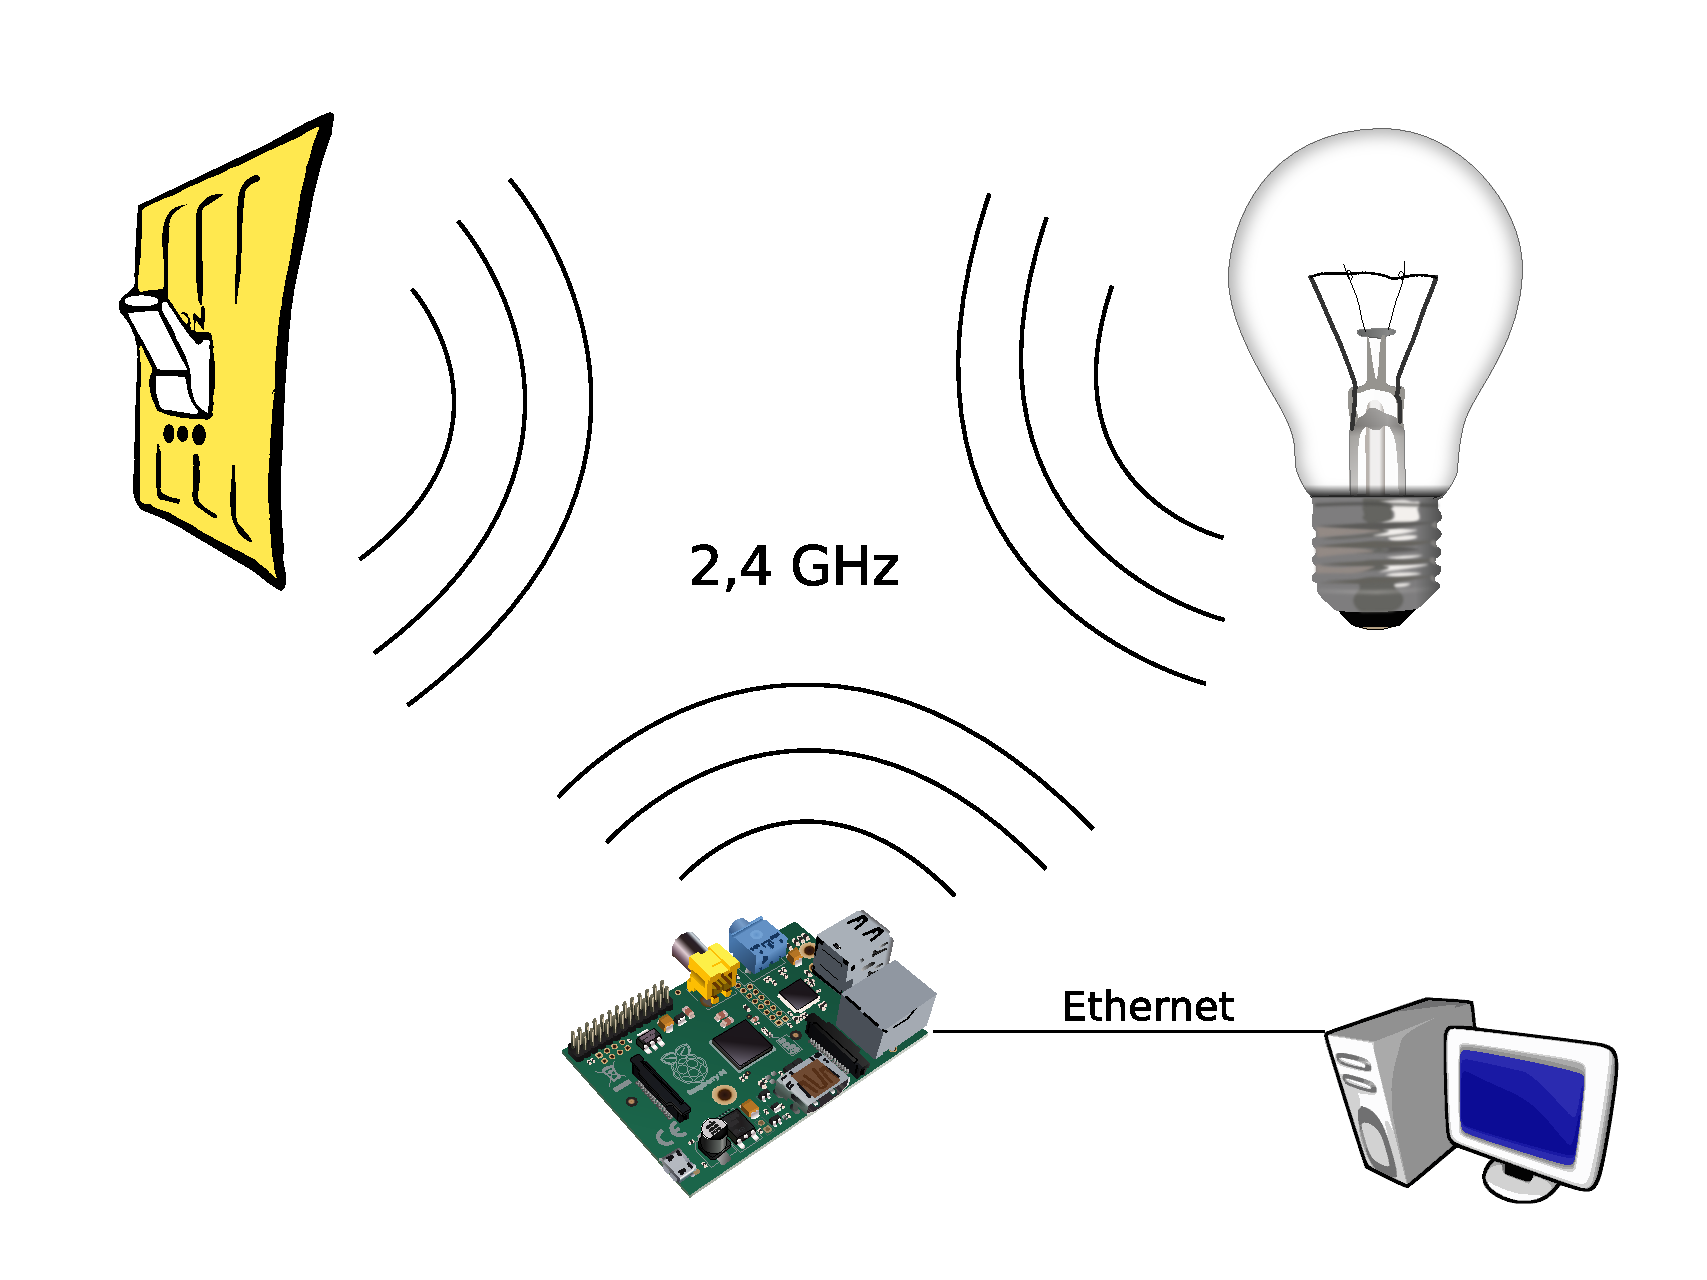
\includegraphics[width=0.5\textwidth]{img/system}
            \caption{Schematische Darstellung der beteiligten Komponententypen}
            \label{fig:comp}
        \end{figure}

        \subsubsection{Sensorknoten}\label{Sensorknoten}
            Sensorknoten sind aus Sicht des Systems im aktuellen Entwurf
            zunächst \enquote{dumm}. Sie enthalten keinerlei Wenn-Dann-Logik
            sondern produzieren ausschließlich Nachrichten mit bestimmten
            Aussagen, z.\,B. \enquote{Ich bin Knoten A und meine erste Taste
            wurde gedrückt}.
        \subsubsection{Aktorknoten}\label{Aktorknoten}
            Aktorknoten ist die eigentliche Aktion-Reaktion-Logik eingepflanzt.
            Sie lauschen auf dem Kommunikationsmedium und warten auf Anweisungen
            ihre möglichen Aktionen auszuführen.

            Dabei sind zwei Varianten vorgesehen:
            \begin{itemize}
                \item Ein Aktor kann eine Nachricht mit seiner eigenen Adresse
                    erhalten. Das bedeutet für ihn, er soll diese Aktion
                    ausführen, unabhängig davon wer das Ereignis ausgelöst hat.
                \item Ein Aktor kann programmiert werden auf bestimmte andere
                    Adressen und Nachrichten zu reagieren.
                    So kann beispielsweise eingestellt werden, dass ein Aktor
                    dann schaltet, wenn er eine Nachricht entdeckt, in der steht
                    \enquote{Ich bin Knoten A und meine erste Taste
                    wurde gedrückt} (siehe oben).
            \end{itemize}

            Durch diese zwei Varianten ist es auf der einen Seite möglich
            dezentral Nachrichten auszulösen und darauf zu reagieren, wobei
            die Auslöser, also die Sensoren selbst relativ einfach aufgebaut
            sein können. Die aufwändigere Logik, welcher Sensor welche Aktion
            auslöst, kann im Aktor implementiert werden.
            Auf der anderen Seite ist es aber trotzdem möglich, das System
            zentral zu nutzen, indem Sensornachrichten von einem zentralen
            Punkt empfangen werden, der anschließend Nachrichten mit konkreten
            Aktoradressen versendet. So können auch Aktoren \enquote{dumm}
            bleiben und können (z.\,B. in einem sehr kleinen, temporären Aufbau)
            ohne jede Programmierung verwendet werden, ohne dass sie von den
            konkreten Sensoren wissen müssen.

            Wie ein solches Gateway aussehen könnte zeigt der folgende Abschnitt.

        \subsubsection{Gateway (derzeit ein Raspberry PI)}
            Ein System, dass unabhängig von äußeren Steuerungsinfrastrukturen
            funktionieren kann, ist für die Akzeptanz im Gebäude wichtig.
            Wenn kein Lichtschalter im Haus mehr funktioniert, weil
            im Keller jemand das falsche Netzwerkkabel gezogen hat,
            wird kein Nutzer recht überzeugt sein.
            Umgekehrt ist es allerdings auch wichtig, Schnittstellen zu
            etablierten Kommunikationsstrukturen zu bieten.
            So ist eine Anbindung an vorhandene IPv4- oder IPv6-Netze
            wünschenswert, sodass auch mächtigere Komponenten integriert werden
            können, die unter Umständen noch weitere Kommunikationsmöglichkeiten
            bieten.

            Momentane Lösung dieses Wunsches ist die Integration eines Computers
            in den cowbus. Die offensichtlichste Möglichkeit war auch bei diesem
            Projekt ein Raspberry PI\footnote{\url{http://www.raspberrypi.org/}},
            der bereits alle nötigen Schnittstellen mitbringt, um direkt das
            $2,4-GHz$-Funkmodul und das vorhandene \ac{LAN} anzuschließen.

            Auf dem Raspberry PI läuft ein kleiner in C++ verfasster Daemon.
            Dieser steuert zum einen das Funkmodul und wartet auf Pakete aus
            dem Funknetz.
            Auf der anderen Seite enthält er einen kleinen Websocket-Server,
            über den von jedem beliebigen PC, der ihn über das \ac{LAN}
            erreichen kann, Pakete in das Funknetz verschickt und aus diesem
            empfangen werden kann.

            Dazu steht eine kleine HTML/JavaScript-Anwendung zur Verfügung,
            die in jedem modernen Browser läuffähig sein sollte.

    \subsection{Paketaufbau}
            \begin{figure}
            \centering
            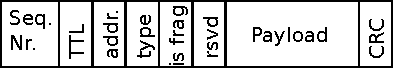
\includegraphics[width=0.5\textwidth]{img/paket}
            \caption{Aufbau der Pakete}
            \label{fig:paket}
        \end{figure}

        Hardware bedingt sind wir für die übertragenen Pakete auf 32\,Byte 
        beschränkt, dazu in der späteren Beschreibung über den Funkchip mehr. 
        Abbildung \ref{fig:paket} zeigt den Aufbau der Pakete. Die Pakete 
        bestehen aus:
        \begin{itemize}
            \item 5 Bit Sequenznummer: aufsteigend, für jeden Teilnehmer individuell
            \item 8-Bit Time To Live: Maximalwert, der beim Weiterleiten decrementiert wird
            \item 11-Bit Adresse: Kontexabhängig ob Sende / Empfangsadresse
            \item 4-Bit Type: Art der Nachricht
            \begin{itemize}
                \item undefined: Reservierter Typ.
                \item event: Ein Ereignis hat stattgefunden, z.\,B. wenn ein Taster gedrückt wurde
                \item program: Einem Aktor eine Funktion zuweisen
                \item get\_name: Den Namen eines Knotens abfragen
                \item get\_state: Statusabfrage
                \item get\_config: Gegenstück zu program, also die Kongiguration abfragen
                \item ping: Abfrage, ob bereits ein Knoten mit angegebener Adresse vorhanden ist
                \item ping\_answer: Antwort auf ping-Nachricht
                \item set\_name: Den Namen eines Knotens festlegen
            \end{itemize}
            \item 1-Bit \enquote{is frag}: dies ist ein einzelnes Bit, das gesetzt ist, falls es sich um eine aufgeteilte Nachricht handelt. Der Fragment Header wird an den Anfang der Payload gesetzt.
            \item 208-Bit Payload, das sind 26 Byte
            \item 16-Bit CRC
        \end{itemize}

\section{Knoten-Prototyp-Hardware}
Tests mit den Discovery-Boards haben gezeigt, dass das Hardware-Konzept tauglich ist.
Aus diesem Grund wurde ein Protoyp entwickelt. \todo{sprachlich wackelig}

\subsection{Anforderungen an den Protoypen}
Ziel des cowbus ist die möglichst einfache Integration in bestehende Installationen.
Aus diesem Grund soll die fertige Platine so bemaßt sein, dass sie in einer Unterputzdose montiert werden kann.
Eine Unterputzdose ist rund und bietet etwa 4\,cm Durchmesser.

Weitere Anforderung ist, dass das Projekt erschwinglich bleibt.
In einer fertigen Installation könnte eine Vielzahl von Knoten verbaut sein, deswegen darf der Preis eines einzelnen Knotens nicht zu hoch werden.
Für die Prototypenplatine wurde ein Ziel von 20 Euro festgelegt.

Abschließend soll die Platine ausreichend sein, um alle grundlegenden Fähigkeiten des Buses zu entwickeln und abzubilden.
Das heißt sie muss sowohl die Anforderungen an einen Sensorknoten (\ref{Sensorknoten}), als auch die an einen Aktorknoten (\ref{Aktorknoten}) erfüllen.

\subsection{Umsetzung des Prototypen}
\todo{Einleitung}

\subsubsection{Energieversorgung}
Eine der Anforderungen ist die Möglichkeit das Board in einer Unterputzdose zu montieren.
Damit gibt es zwei Möglichkeiten der Energieversorgung.
Wenn in der Dose Netzspannung verfügbar ist, kann die Energie hieraus bezogen werden.
Andernfalls muss das Board aus einer Batterie versorgt werden.

Für den Prototypen wurde die letztere Option gewählt.
Um ein Netzteil für Unterputzdosenmontage zu realisieren, müsste eine stark integrierte Baugruppe, welche bei Netzspannung arbeitet, entworfen werden.
Dies ist im Rahmen dieses Projektes nicht umsetzbar.

Aus diesem Grund wurde eine Energieversorgung per Batterie umgesetzt.
Dazu kommt der Boost-Converter TPS61221 von \emph{Texas Instruments} zum Einsatz.
Dieser zeichnet sich durch einen niedrigen Ruhestrom von $0,5 \mathrm{\mu A}$ aus.

Die Planung sah vor, die Schaltung auch optional über USB zu versorgen.
Dieser Zustand ist über Jumperstellungen auswählbar.
Das Datenblatt des Wandlers wurde dazu fehlerhaft interpretiert, da dieser nur 5V-tolerant ist.
Damit ist es in der aktuellen Hardware-Revision nicht möglich die Baugruppe über USB zu versorgen.
Als Abhilfe ist für die nächste Revision ein zusätzlicher LDO-Regler vorgesehen.

\subsubsection{Prozessor}
Die Wahl eines geeigneten Mikrocontrollers wurde früh auf 32bit-Architekturen eingeschränkt. Am heutigen Markt ist der preisliche Unterschied nahezu irrelevant. Zudem ist die Rechnenleistung der \enquote{größeren} Plattformen meist besser. Der gewählte Chip ist der STM32F030C8T6. Es war der günstigste, der den Anforderungen von Riot und denen des entworfenen Protokolls genügt. Ausserdem ist die Toolchain der ARM-Prozessoren von STM gut ausgereift.
Für den verwendeten Microcontroller ist ebenfalls ein Discovery-Board verfügbar, sodass auch hier wieder der Entwicklungsstart ohne die Platine begonnen werden konnte.

\subsubsection{Funkmodul}
Auf dem Prototyp wird der gleiche Chip, der auch in den Vorversuchen funktioniert hat, verwendet: der nrf24l01+. Der Funkchip arbeitet, wie oben bereits erwähnt, im 2,4GHz ISM-Band.
%\todo{kann das weg?: * Wahl des Funkchips (hier 32-Byte Beschränkung, GFSK und Frequenzbänder/Bandbreiten)}
%ja, definitiv!

\subsubsection{Peripherie}
Gemäß den Anforderungen ist der Prototyp mit entsprechender Peripherie bestückt.
Zum einen sind drei Taster angeschlossen, um einen grundlegenden Sensor zu modellieren.
Zum anderen befindet sich auf dem Board eine RGB-LED, welche eine primitive Form eines Aktors darstellt.

Für zukünftige Features ist ein Summer vorgesehen.
Dieser wird mit einem N-MOSFET angeschalten.
Der Summer ist dazu vorgesehen, einzelne Knoten während der Konfiguration zu erkennen.

Um Daten wie die Konfiguration des Knotens dauerhaft zu speichern, ist an den Mikrocontroller ein EEPROM über SPI angeschlossen.
Die SWD-Funktionalität des Controllers ist in Form einer Cortex-M-Debugschnittstelle herausgeführt.

    \todo{ausmisten: Platine, Aufbau, Designentscheidungen, ...}

\section{Software}
    Um die Entwicklungszyklen kurz zu halten haben wir uns dafür entschieden
    ein Betriebssystem einzusetzen, das Grundfunktionalitäten bereits
    zur Verfügung stellt.

%    \subsection{Kommunikationsstruktur: Nachrichtenbasiert, jeder Knoten entscheidet anhand Adresse ob er interessiert ist am Inhalt}
    \subsection{RIOT -- The friendly Operating System for the Internet of Things.\cite{RIOT}}
        RIOT OS möchte ein Betriebssystem für eingebettete Systeme sein,
        das einfach zu bedienen und ressourcensparend ist und dabei speziell
        auf Internet-of-Things-Anwendungen abzielt. Es bringt viele Definitionen
        für verbreitete Entwicklungs- und Prototyping-Boards mit, darunter die
        STM32F*-Discovery-Serie.
        Die Abstraktion von hardwareabhängigem Code vom eigentlichen Kernel
        ermöglicht eine weitgehend getrennte Entwicklung von Funktionalität und
        Hardwareunterstützung.

        Theoretisch genügt der Austausch des Hardware Abstraction Layers,
        um den RIOT-Code von einer Plattform auf eine andere zu portieren.

    \subsection{RIOT und cowbus}
        In der Praxis hat sich diese Abstraktion aber nur als teilweise sauber
        implementiert herausgestellt. Leider ist vor allem der Netzwerkstapel
        sehr unübersichtlich aufbaut, nicht sauber getrennt und vor allem kaum
        dokumentiert. Allein diese Tatsache hat die Entwicklung des cowbus stark
        verzögert, weil lange nicht klar war, wie viel möglich ist.
        Prinzipiell bietet RIOT auch Implementierungen für Protokolle oberhalb
        der MAC-Schicht. So sind z.\,B. Teile von 802.15.4 sowie diverse
        Routingprotokolle implementiert. Leider sind vor allem erstgenannte
        Funktionen nicht sauber getrennt, sondern Funkchip-abhängig in den
        Code zur Ansteuerung der Netzwerkschnittstelle gemischt, sodass eine
        Wiederverwendung der Codes kaum sinnvoll möglich ist.

        Der Netzwerkstapel ist zum Zeitpunkt der Fertigstellung dieser
        Beschreibung allerdings in einem Refactoringprozess,
        sodass sich das möglicherweise in absehbarer Zeit ändert und nicht
        abschließend darüber geurteilt werden soll.

        Letztendlich bietet die Nutzung von RIOT als Betriebssystem trotzdem
        große Vorteile. Vor allem jetzt, nachdem die Portierung auf die eigene
        Plattform fast abgeschlossen ist, erwarten wir deutlich kürzere
        Entwicklungszyklen.

    \subsection{Packet Handler}
        Wir nutzen im Moment nur die unterste Schicht von RIOTs Netzwerkstapel.
        Sobald ein Paket empfangen wurde, löst der Funkchip einen Interrupt aus,
        der von RIOTs Packet Handling abgefangen wird. Die Pakete werden in eine
        Warteschlange geschoben und der Anwendung wird signalisiert,
        dass ein Paket empfangen wurde.
        Die Anwendung besitzt einen eigenen Paketempfangsthread,
        der die Nachrichten aus der Warteschlange abholt und verarbeitet.


    \subsection{Kritik}
        Die Entscheidung, ob ein Betriebssystem zum Einsatz kommt,
        wurde sehr bald getroffen. Verleitet von den vollmundigen Versprechen,
        die RIOT auf seiner Homepage macht, schien es die perfekte Lösung für
        unser Vorhaben zu sein. In der Praxis hat sich sehr schnell gezeigt,
        dass RIOT nicht so bunt ist, wie es seine eigenen Werbung malt.
        Anfangs versuchten wir ein CC1101-Funkmodul mit einem
        STM32F3-Discovery-Board zu betreiben. Wie sich herausstellte,
        bietet RIOT zwar einen Treiber für das Modul und unterstützt die
        PLattform an sich, konkret war allerdings kein SPI-Treiber für das Board
        implementiert. Solche Rückschläge häuften sich und kosteten viel Zeit.
        Trotz allem hoffen wir, dass sich die Wahl in Zukunft auszahlt und
        die bestehende Plattform so viel Arbeit abnimmt, dass sich die
        bisher investierte Zeit auszahlt.


\section{Ausblick}
    Zum jetzigen Zeitpunkt existieren in erster Linie Einzelteile,
    die gemeinsam betrachtet aufzeigen, welche Möglichkeiten sich bieten
    und Potential erahnen lassen.

    \subsection{Hardware}
        Der nächste Schritt wird die vollständige Inbetriebnahme der eigenen
        Prototyp-Schaltung sein, sodass zukünftige Entwicklungen nicht mehr
        auf einem Discovery-Board getestet werden müssen, sondern direkt auf
        der Zielhardware laufen können.

    \subsection{Medienzugriffsverfahren}
    Im aktuellen Stand der Entwicklung ist der Zugriff auf das Funkmedium in 
    keiner Weise koordiniert. Sobald ein Knoten Daten zum verschicken hat, 
    sendet er sie auch aufs Funkmedium. 

    Da auf das Funkmedium mehrere Knoten gleichzeitig zugreifen, ist ein 
    Medienzugriffsverfahren notwendig. Diese beschreiben den Ablauf des 
    Kanalzugriffs und können somit Konflikten vorbeugen oder diese zuindest 
    erkennen und eine Lösung dafür einleiten. Ein Verfahren, das Konflikte 
    vorbeugen soll ist Carrier Sense Multiple Access with Collision Avoidance 
    (CSMA/CA, dt.: Mehrfachzugriff mit Trägerprüfung und Kollisionsvermeidung). 
    CSMA/CA ist für ein paketvermitteltes lokales Netzwerk mit unregelmäßigem 
    Datenaustausch aller Teilnehmer konzipiert worden. Dies entspricht auch 
    diesem Anwendungsfall.
    Der Mehrfachzugriff mittels CSMA/CA Verfahren auf ein Medium beinhaltet das 
    Carrier Sensing (dt. Trägerprüfung). Dies bedeutet, dass ein Sender lauscht, 
    ob der Kanal frei ist, bevor er sendet. Der Sender wartet, falls ein zweiter 
    Teilnehmer sendet, bis dieser seine Daten verschickt hat. Der Sender beginnt 
    nicht sofort im Anschluss das Senden. Hierbei wäre die Gefahr zu groß, dass 
    andere Teilnehmer, die ebenfalls auf die Freigabe des Funkkanals gewartet 
    haben, mit ihm gleichzeitig das Senden beginnen. Der Teilnehmer, der senden 
    möchte wartet in diesem Fall ein zufälliges Zeitintervall und empfängt nach 
    dieser Zeit erneut. Ist der Kanal dann belgt, wartet er erneut eine 
    zufällige Zeit. Ist der Kanal bei Ablauf der zufälligen Zeit frei, so sendet 
    er.
    Die Besonderheit des CSMA/CA Verfahrens stellt die Kollisionsvermeidung dar. 
    Steht ein Rahmen zur Übertragung an, so wird geprüft, ob das Medium belegt 
    ist. Ist es frei, so wird der Rahmen nach einem kurzen Zeitraum, der als 
    DIFS (Distributed Inter-Frame Space) bezeichnet wird, gesendet. DIFS stellt 
    den minimalen zeitlichen Abstand zwischen zwei gesendeten Datenrahmen auf 
    einem Übertragungsmedium dar. Ist der Kanal jedoch belegt, wählt die Station 
    eine zufällige Wartezeit. Diese wird heruntergezählt, sobald der Kanal frei 
    ist. Während anderer Übertragungen bleibt diese Zeit eingefroren. Sobald die 
    Zeit abläuft wird der gesamte Rahmen übertragen. 
    Obwohl zwei Teilnehmer gleichzeitig das Medium als frei detektieren und das 
    Senden anfangen, können sich deren Daten bei einem dritten Teilnehmer 
    überlagern und unbrauchbar werden. Bei gezielter Übertragung an einen 
    Nachbarn kann an dieser Stelle auf eine Empfangsbestätigung gewartet werden 
    und der Rahmen erneut gesendet werden, falls diese nicht eintrifft. In 
    unserem Netz ist es bislang jedoch noch nicht vorgesehen, dass ein Knoten 
    seine Nachbarn kennt oder auf Empfangsbestätigungen wartet. 

    \subsection{Kompression der Payload}
    Codierung der Zeichen in der Payload: 
    In der Payload sollen bei den Pakettypen get\_name und set\_name für den 
    menschen lesbare Buchstaben als Name eines Knoten übertragen werden. Bei 
    unkomprimierter Übertragung mittels Ascii Zeichen, also 8~Bit pro Zeichen, 
    wären bei einer maximalen Payload von 208~Bit nur 26~Zeichen möglich. Zur 
    Kompression des Knotennamens gibt es hier im Allgemeinen zwei Möglichkeiten. 
    Zum einen können aufgrund der Buchstabenwahrscheinlichkeit in einer 
    bestimmten Sprache ein oder mehrere Buchstaben durch Symbole ersetzt werden 
    (z.\,B. mittels Huffmann oder Vektor-Huffman Codierung). Bei diesem Verfahren 
    entstehen allerdings bei gleich langen Namen unterschiedlich lange Paylods. 
    Da die maximale Anzahl von Buchstaben nicht mit den Buchstaben selbst 
    variieren soll, ist dieses Verfahren ungeeignet. Die zweite Möglichkeit ist 
    die Anzahl an möglichen Zeichen beschränken. Es sind für Namen von Knoten 
    also nur noch Zahlen, Buchstaben und 4~Sonderzeichen (Null-Terminator, 
    Leerzeichen, at-Zeichen, Unterstrich) zugelassen. Dies ergibt 40~Zustände 
    pro Zeichen, die wir als gleich wahrscheinlich annehmen. Bei 40~möglichen 
    Zuständen ergibt sich ein Informationsgehalt von $$log_{2}(40) = 5,32~bit$$. 
    Für drei Zeichen ergibt sich ein Informationsgehalt von 
    $$log_{2}(40^3) = 5,32 \cdot 3~bit < 16~Bit.$$ Es können also 3~Zeichen 
    in 2~Byte codiert werden. Mit 8~Bit pro Zeichen wären in der Payload 
    26~Zeichen möglich gewesen, mit Reduzierung der Zustände sind nun 39~Zeichen 
    möglich.
    Anschaulich gesehen ergeben sich mit 40~Möglichkeiten pro Zeichen bei 
    3~Zeichen $40^3 = 64000$ Möglichkeiten. Mit 16~Bit können 65536~Zustände 
    abgebildet werden. 
    Es werden drei Zeichen ($x_{1}$, $x_{2}$, $x_{3}$) in ein Symbol gepackt. 
    Dieses Symbol kann durch folgendes Polynom berechnet werden:
    $$Symbol = x_{1} \cdot 40^{0} + x_{2} \cdot 40^{1} + x_{3} \cdot 40^{2}$$
    Die Decodierung erfolgt über folgende Gleichungen:

    $$x_{1}=Symbol \,\, \% 20$$

    $$x_{2} = \frac{Symbol - x_{1}}{40} \% 40$$
    
    $$x_{3} = \frac{Symbol - (x_{1} + x_{2} \cdot 40)}{40} (\% 40)$$

    \subsection{Routing}
        Damit die Nachrichten, die ein Knoten losschickt, auch ihr Ziel 
        erreichen ist eine Wegewahl und damit eine Strategie zur Weiterleitung 
        der Pakete erforderlich. Ein Sensor schickt jedoch nur seine 
        Zustandsänderung ins Netz. Welcher und wie viele Aktoren auf diese 
        Nachricht reagieren weiß der Sensor jedoch nicht. Die Nachrichten müssen 
        daher alle Knoten erreichen, mit anderen Worten: es gibt nur 
        Broadcast-Nachrichten. Ein Routingverfahren für eine effiziente Wegewahl 
        ist daher nicht erforderlich.
        Da es nur Broadcast-Nachrichten gibt, werden die Nachrichten über fluten 
        verbreitet. Ein Sensor schickt eine Nachricht an seine Nachbarn. Diese 
        schicken die Pakte wieder weiter und so verbreitet sich die Nachricht im 
        Netz. Damit jedoch die Nachricht nicht zwischen zwei Knoten hin- und 
        her pendelt, merkt sich jeder Knoten den Header jedes Paketes, das er 
        weiter leitet in einem FIFO-Puffer, damit er das selbe Paket kein 
        zweites Mal weiter leitet.
        

    \subsection{Verschlüsselung}
    Um das System im eigenen Haus gegen Angriffe von aussen zu schützen soll in 
    späteren Versionen eine Verschlüsselung erfolgen. 




\todo{kritische Auseinandersetzung mit getätigten Design-Entscheidungen}

\section{Zusammenfassung}

\todo{fehlt}

\section*{Abkürzungen}
\renewcommand{\IEEEiedlistdecl}{\IEEEsetlabelwidth{CSMA/CA}}
\begin{acronym}
    \acro{6LoWPAN}{IPv6 over Low power Wireless Personal Area Network}
    \acro{CSMA/CA}{Carrier Sense Multiple Access with Collision Avoidance}
    \acro{LAN}{Local Area Network}
    \acro{openHAB}{open Home Automation Bus}
\end{acronym}
\renewcommand{\IEEEiedlistdecl}{\relax}% remember to reset \IEEEiedlistdecl


\comment / *
\listoffigures
\clearpage

\listoftables
\clearpage
* /

\bibliographystyle{IEEEtran}
\bibliography{IEEEabrv,projektdoku_cowbus}

\end{document}
